%!TEX root=../main.tex
\section{Application} % (fold)
\label{sec:application}

\textcolor{red}{We apply the method to the sport science field. We use the Python package \texttt{nba\_api}\footnote{\url{https://github.com/swar/nba_api/}} to access the APIs of \url{nba.com} and all the data from NBA games. The dataset consists of all the shots location from every games between the season $2018-2019$ and $2022-2023$. We only keep the players who made more than $1000$ shots during these five seasons. There are $131$ such players resulting in $493723$ shots taken and $234941$ shots made. We remove the impossible shots (not on the field), we have $492621$ shots left. We estimate the shooting density for each player using 2-dimensional kernel density estimation using bandwidth estimation with Silverman's rule \cite{silvermanDensityEstimationStatistics1986}. The density is estimated on a regularly spaced grid of $51 \times 51$ points.}

\textcolor{red}{A MFPCA is run on the data. Figure \ref{fig:shoots_decomposition} shows examples of the shooting densities of Stephen Curry and Kevin Durant and their first five functional principal components.}
\begin{figure}
    \centering
    \begin{subfigure}[b]{0.4\textwidth}
        \centering
        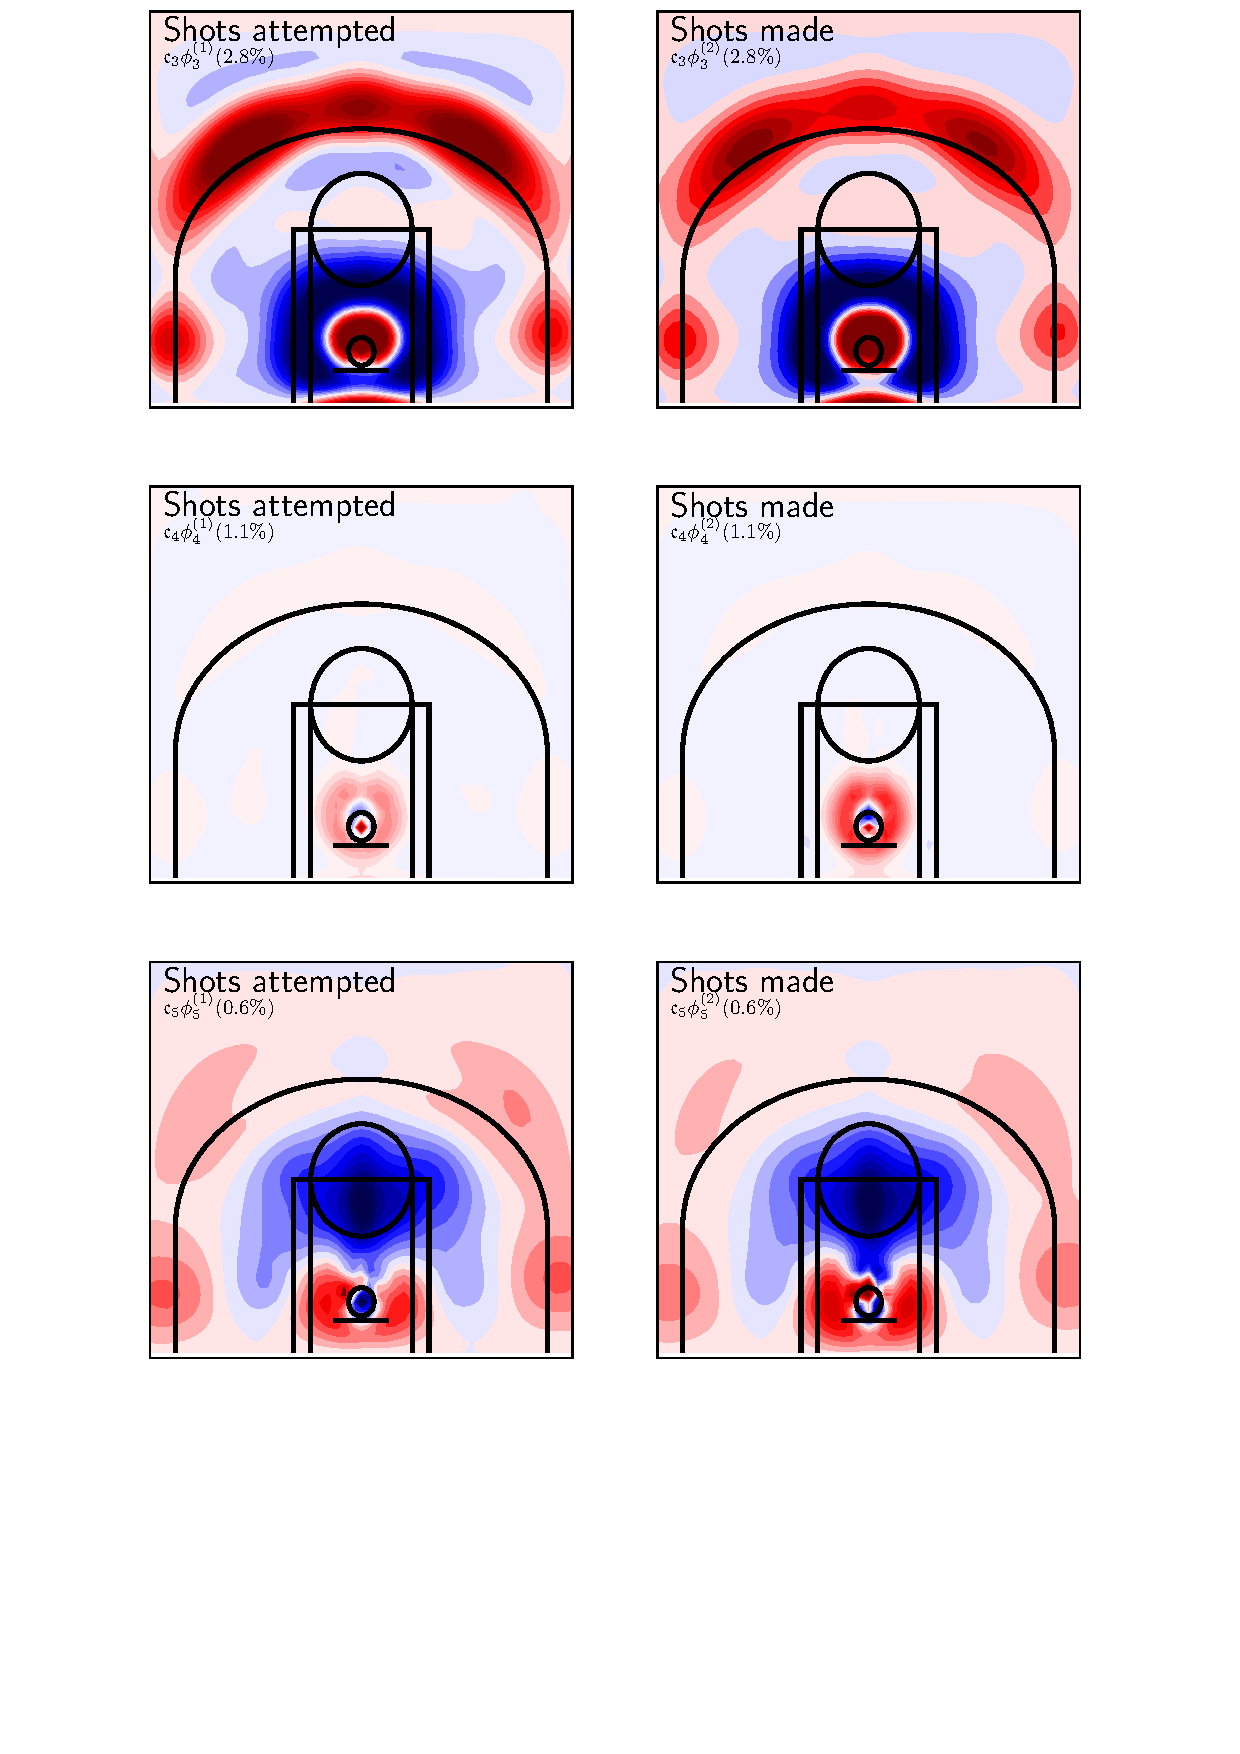
\includegraphics[width=\textwidth]{figures/curry_decomposition.pdf}
        \caption{Stephen Curry}
        \label{fig:curry_decomposition}
    \end{subfigure}
    \hfill
    \begin{subfigure}[b]{0.4\textwidth}
        \centering
        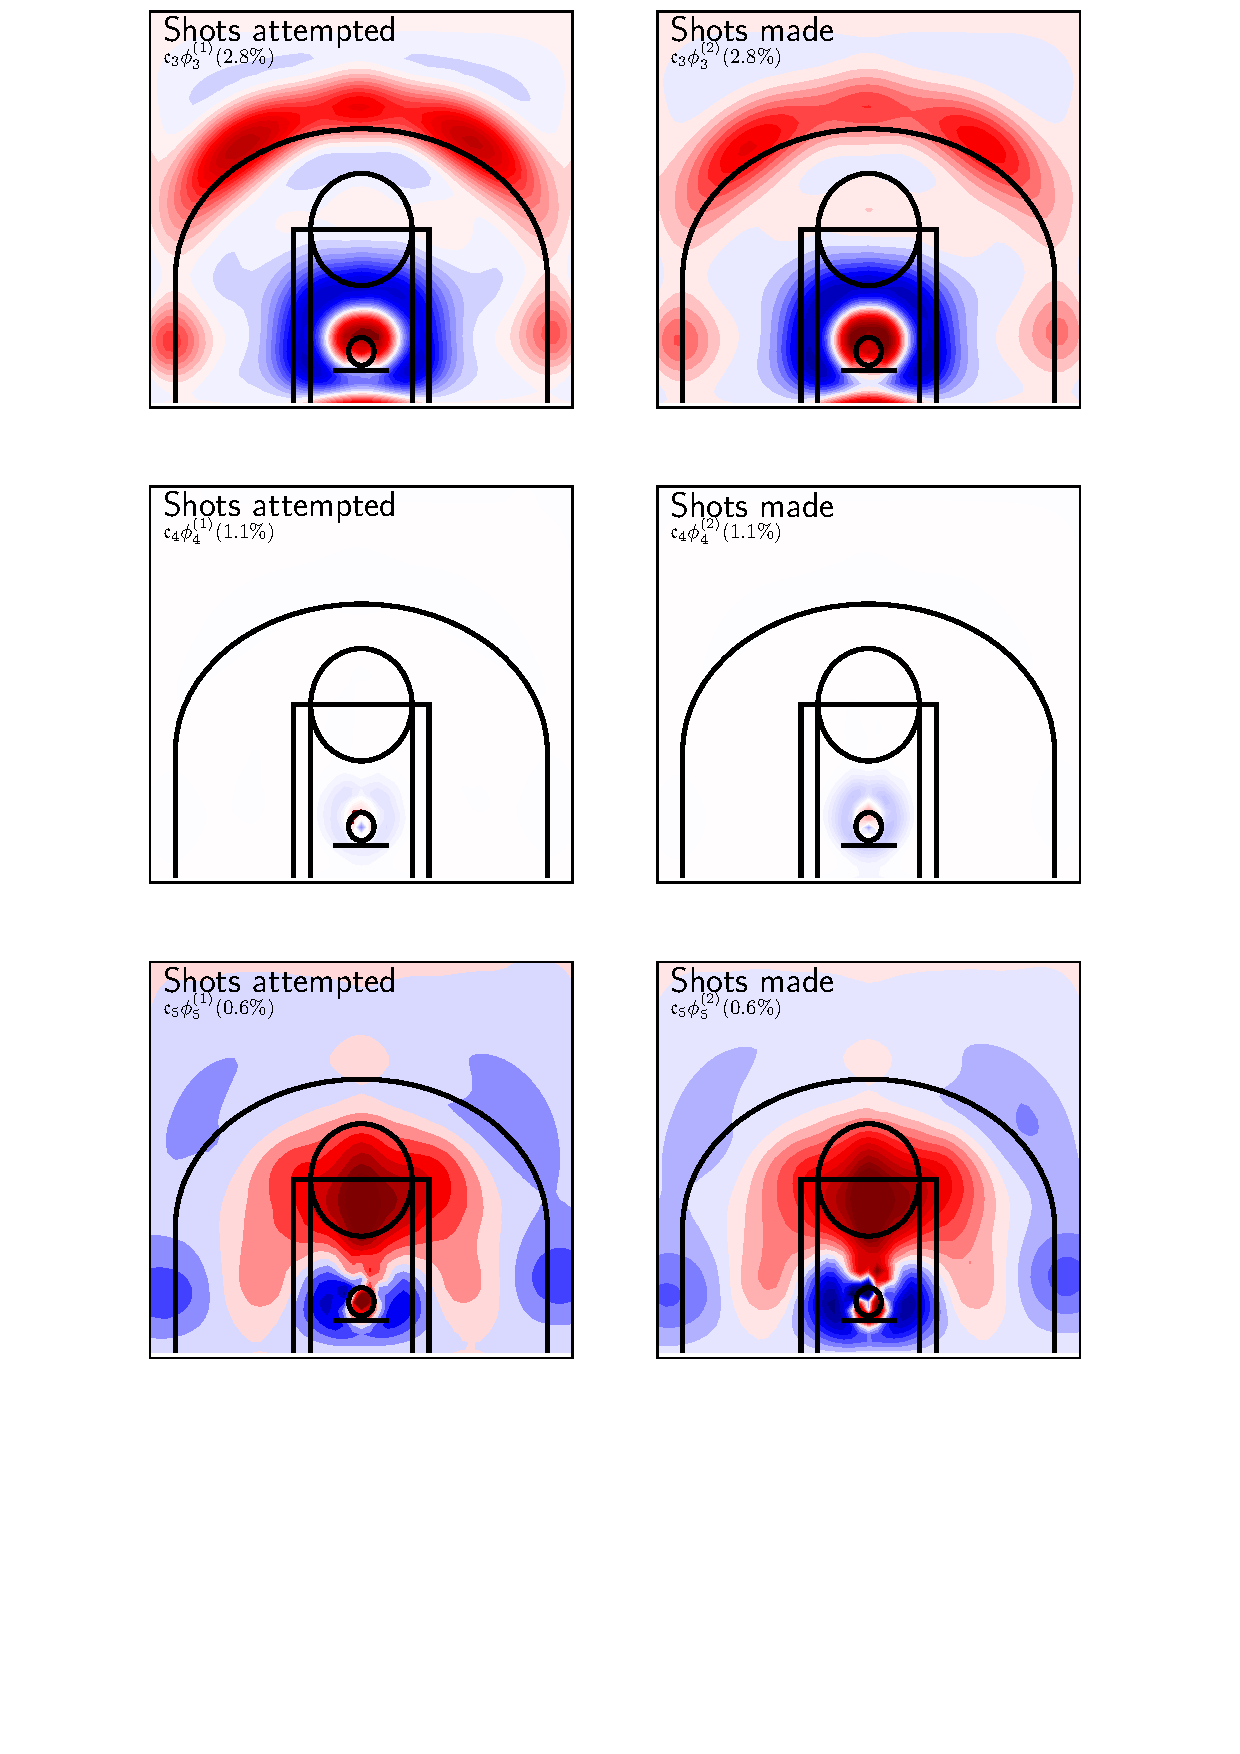
\includegraphics[width=\textwidth]{figures/durant_decomposition.pdf}
        \caption{Kevin Durant}
        \label{fig:durant_decomposition}
    \end{subfigure}
    \caption{Decomposition for Stephen Curry and Kevin Durant.}
    \label{fig:shoots_decomposition}
\end{figure}

% section application (end)